% This is LLNCS.DOC the documentation file of
% the LaTeX2e class from Springer-Verlag
% for Lecture Notes in Computer Science, version 2.4
\documentclass{llncs}
\usepackage{llncsdoc}
\usepackage{color}
\usepackage{graphicx}
\usepackage{subfigure}
\usepackage{listings}
\usepackage{bold-extra}
\usepackage{wrapfig}
\usepackage{float}
\usepackage{algorithm2e}
\usepackage[backgroundcolor=pink!40]{todonotes}
%



\begin{document}
\lstset{ 
	language = [AspectJ]Java,
  basicstyle=\ttfamily\footnotesize,
  numbers=left,
	numberstyle=\tiny\color[rgb]{0.25,0.25,0.25},
  firstnumber=auto,
	breaklines=true,
  tabsize=2,
	emph={aspect,declare, adapter, instance, pointcut, adaptee, adapts, select, UNTIL,pc,name, instanceType, exp, removeExp}, 
	emphstyle=\textbf,
	stringstyle=\textsf,
	showstringspaces= false,
	frame=single
	}

\title{SLE2012}

\author{Kardelen Hatun \and Christoph Bockisch \and Mehmet Ak\c{s}it}
\institute{TRESE, University of Twente \\ 7500AE Enschede \\ The Netherlands \\
\url{http://www.utwente.nl/ewi/trese/}\\
\email{ \{hatunk,c.m.bockisch,aksit\}@ewi.utwente.nl}
}

\maketitle

\section{Introduction}
In object-oriented programming (OOP), objects encapsulate state and behavior; objects also have a life-cycle, which means that the same object can play different roles at different times. And which role an object is currently playing is important as it can affect the object’s own behavior or how objects are handled. Often the shift from one life-cycle phase to another is implicit, e.g., determined by passing an object from one client to another. In this paper, we propose a new language mechanism for declaratively specifying life-cycle phases and for exposing the set of objects which are currently in a specific phase. This declarativity allows us to give guarantees about these sets like subset relationships, as well as to perform compile-time checks like warning about sets that will always be empty.

As an example of different relevant phases in the life-cycle of objects, consider an online store application. Assume that the offered products are objects in the program and that specific budget plans should be offered for products depending on their life-cycle phase. A first example of such a phase is a period during which a product is in the wish-list of any customer; this phase begins when ``product'' object is added to the ``wish-list'' property of a ``customer'' object and it ends when it is removed from this property. A second example is the phase when an object is out of stock. Thus, we defined two sets of objects: the set of objects into which at least one customer is interested and the set of objects that are sold out. Finally, the shop owner may be interested in the intersection of these sets and give priority to reordering the corresponding products.

To be able to process the objects which are currently in a relevant life-cycle phase, bookkeeping is required to keep track of the set. To separate this bookkeeping code from the business logic of the program, aspect-oriented programming (AOP) is a well known technique. But current aspect-oriented languages do not offer dedicated mechanisms for selecting \emph{sets of objects}. These languages do not support a \emph{declarative specification} of the objects belonging to a life-cycle phases; instead an \emph{imperative implementation}, following always the same pattern, is required for collecting those objects 

A consequence of such an imperative solution, besides all the negative effects of hand-writing boilerplate code, is that automatic reasoning becomes practically impossible. TODO elaborate

To offer better support for processing objects according to their life-cycle phase, we propose a language construct that builds on the technology of aspect-orientation. In AOP, \emph{pointcuts} select sets of so-called \emph{join points} which are points in time during the execution of the program. We borrow the terminology and provide \emph{instance pointcuts} to select sets of objects based on the execution history.

\todo[inline]{elaborate ... explain a bit the language, and the different features}
%Components interact through their interfaces. In component-based systems, there are cases where a certain functionality is provided by a third-party software which usually comes with an incompatible interface, which makes connecting new components and the existing components a challenge.  An important requirement of \emph{binding} two components is to encapsulate the binding declarations in a separate module, while leaving the bound components untouched.  In this study we present a language which satisfies this requirement and offers a reusable, maintainable and concise way of expressing binding.
%
%Our language is composed of two main structures; \textbf{instance pointcuts} and \textbf{adapter declarations}. Instance pointcuts are specialized pointcuts, which are used to capture the instances of a type, which at some point in their life cycle become relevant. This can be creation of the instance, calling a certain method on the instance or passing the instance as an argument. The conditions for becoming relevant is defined in the pointcut expression. Adapter declarations provide a declarative syntax for implementing object adapters, where the objects to be adapted are selected by instance pointcuts. The benefit of our approach partly comes from utilization of Aspect Orientation (AO), which allows modularization of binding concern. But the major benefit is due to the marriage of two new language concepts which take object adapters to a new level. 
%
%The traditional object adapter is shown in Figure \textsl{(objectadapter)}. Instance pointcuts provide means to select a subset of instances that belong to a specific type. It is also possible to select all subtype instances of a supertype, since the instance pointcut captures dynamic types. In adapter declarations this subset can be adapted by referring to the instance pointcut. An adapter declaration consists of a unique name, an instance pointcut reference and a list of interfaces to be implemented. The interface methods are overriden in the adapter declaration, referring to its \emph{adaptee} where adaptee is an instance belonging to the set of instances selected by the instance pointcut. When an instance pointcut expression matches a join-point and that instance pointcut is referred to by an adapter declaration, then an adapter instance is automatically created containing the instance in the matched join-point.  In an OO approach this would require adapter instantiations at various points in the code, which will cause tangling of adapter instantiation concern. 
%
%It is also possible to have an inheritance hierarchy among adapters, by defining \emph{abstract adapters}. Abstract adapters do not have to implement all the interfaces they declare, whereas \emph{concrete adapters} have to provide an implementation for every interface they declare or for the unimplemented interface declared by their super-adapter. Concrete adapters can also override the implementations of their super-adapters. This abstraction mechanisms leads to maintainable adapters and reduce programming efforts should the components evolve.
%
%The AO nature of our approach allows all of these features to be encapsulated in an aspect. The concern is localized therefore there's no scattering and tangling. Moreover a run-time library for querying and retrieving adapters is created. With this library the user can query adapters by using an instance, a type, an adapter name or a combination of these as a key. This allows accessing adapters in a flexible way, whereas in the traditional OO implementation, it is only possible to access an adapter is by using its instance name.  

\section{Motivation}
\todo[inline]{Introduce Online Shop example in detail, introduce relevant structures, identify event variations for object (Product can be passed as an argument etc)}
\todo[inline]{Explain what cannot be done with current approaches}
\todo[inline]{Explain briefly How instance pointcuts can remedy the situation}

\section{Instance Pointcuts}

An object can be accessed from multiple modules during its life-cycle. Objects are categorized according to their \emph{types}. This is a structural categorization and it does not give any information about the events that object participates in. However, grouping objects according to another criteria such as, the class they were initialized in or being passed as an argument to a certain method would only be possible by inserting code at those particular points, which would litter the code.  
Instance pointcut is a declarative language construct that is used to select a group of objects of a specific type. The result of the selection is a \emph{set}, hence it cannot contain the same object more than once. Instance pointcuts provide the ability to select objects over a period marked by events in their life-cycle, modularizing the object selection concern. It also provides a mechanism to construct a set of objects according to relevant events, the places in application those events take place and object state at a certain point in execution. Instance pointcuts lets the user to make focused selections,therefore manage the system at a finer level.

A concrete instance pointcut definition consists of a left hand-side and a right-hand side. In the left hand side the pointcut's name and the instance type of interest is declared. Instance pointcuts cannot declare variables, it only has a single implicit variable called \texttt{instance} of the declared instance type. In the right hand side a pointcut expression describes the desired join-points and then binds the exposed object as a member of the instance pointcut's set, which is represented by the variable \texttt{instance}.  It is also possible to declare an abstract instance pointcut, by leaving out the right hand side and placing the \emph{abstract} modifier at the beginning of the declaration.
 %, caption={A simple instance pointcut}, label={lst:simpleip}]%
%\vspace{-15}
\begin{lstlisting}[float=h!]
instance pointcut customers<Customer>: call(Session.createCustomer(..)) && returning(instance)
\end{lstlisting}
%\vspace{-15}

The instance pointcut above shows a basic example. The left-hand side of the instance pointcut indicates the pointcut is called \texttt{customers} and it is interested in selecting the \texttt{Customer} objects. On the right-hand side, the pointcut expression selects the join-points where \texttt{Customer} is returned by the \texttt{createCustomer} of the class \texttt{Session}. The returned instances are exposed and bound by the \texttt{returning} clause to the \emph{implicit variable} \texttt{instance}, which represents a member of \texttt{customers}' set. After selecting a set of objects, instance pointcuts offer ways to manipulate this set. 


\todo[inline]{small introduction and maybe section outline}
\missingfigure{Static Structure of instance pointcuts}

\subsection{Features}

\subsection{Basic Syntax}
\missingfigure{Simple example}

\subsection{Supported AspectJ Predicates}

\todo[inline]{Here we will discuss which predicates we support, with additional explanation of the returning clause}

\subsection{before / after Statements}\\*

\todo[inline]{How to use them and invalid combinations}
\todo[inline]{What is the default behavior if they are not explicitly defined}
\todo[inline, color =green!40]{Additional checks?}
\missingfigure{Example using before after statements}

\subsection{Deselection}

\todo[inline]{How to deselect instances, what are possible checks?}
\missingfigure{Example using UNTIL clause, also incorporating before/after}

\subsection{Instance Pointcut References}

\todo[inline]{how to reference instance pointcuts}
\todo[inline]{Type-refined references}

\subsection{Instance Pointcut Composition}

\subsection{Subsets}

\todo[inline]{Explain what type of relationships subsets stand for}
\todo[inline]{Paragraph: subsetting by type refinement}
\todo[inline]{Paragraph: subsetting by narrowing down the pointcut expression with additional predicates}
\missingfigure{Examples of subsetting, type refinement, additional predicates and both}

\subsection{Supersets}

\todo[inline]{Explain what type of relationships supersets stand for}
\todo[inline]{Paragraph: superset by composing multiple instance pointcuts refer to union operation}
\todo[inline]{Paragraph: superset by composing an instance pointcut with an expression}
\missingfigure{Examples of supersetting}

\subsection{Union, Intersection and Set Difference}
\todo[inline]{Define these operations and give simple examples}



%\section{Instance Pointcuts}
%\label{sec:ip}
%
%An object can be accessed from multiple modules during its life-cycle. Objects are categorized according to their \emph{types}. This is a structural categorization and it does not give any information about the events that object participates in. However, grouping objects according to another criteria such as, the class they were initialized in or being passed as an argument to a certain method would only be possible by inserting code at those particular points, which would litter the code.  
%
%For example, in an online-store application, during a purchase action a \emph{product} object is used by modules like product manager, shopping bag, shipping info and payment process. For analysis purposes, we would like to count the purchases that are made from a particular city. Later according to our analysis results, we may want to apply a discount to that product type and apply further discount if 3 items of that product is present in the shopping bag. To perform these operations we need to insert code to multiple modules to capture relevant events, which cross-cuts the original module functionality.
%
%Instance pointcut is a declarative language construct that is used to select a group of objects of a specific type. The result of the selection is a \emph{set}, hence it cannot contain the same object more than once. Instance pointcuts provide the ability to select objects over a period marked by events in their life-cycle, modularizing the object selection concern. It also provides a mechanism to construct a set of objects according to relevant events, the places in application those events take place and object state at a certain point in execution. Instance pointcuts lets the user to make focused selections,therefore manage the system at a finer level. For the online store example, instance pointcuts can select necessary object for the relevant criteria such as shipping destination, price etc. in a single concise pointcut declaration. 
%
%A concrete instance pointcut definition consists of a left hand-side and a right-hand side. In the left hand side the pointcut's name and the instance type of interest is declared. Instance pointcuts cannot declare variables, it only has a single implicit variable called \texttt{instance} of the declared instance type. In the right hand side a pointcut expression describes the desired join-points and then binds the exposed object as a member of the instance pointcut's set, which is represented by the variable \texttt{instance}.  It is also possible to declare an abstract instance pointcut, by leaving out the right hand side and placing the \emph{abstract} modifier at the beginning of the declaration.
 %, caption={A simple instance pointcut}, label={lst:simpleip}]%
%\vspace{-15}
%\begin{lstlisting}[float=h!]
%instance pointcut shapes<Shape>: call(Shape+.new(..)) && within(ShapeGenerator1) && returning(instance)
%\end{lstlisting}
%\vspace{-15}
%
%The instance pointcut above shows a basic example. The left-hand side of the instance pointcut indicates the pointcut is called \texttt{shapes} and it is interested in selecting the \texttt{Shape} objects. On the right-hand side, the pointcut expression selects the join-points where \texttt{Shape} or its subtypes are instantiated (\textbf{+} operator indicates subtypes are selected, for a complete documentation please refer to ...) \emph{within} the class \texttt{ShapeGenerator1}. The created instances are exposed and bound by the \texttt{returning} clause to the \emph{implicit variable} \texttt{instance}, which represents a member of \texttt{shapes}'s set. After selecting a set of objects, instance pointcuts offer ways to manipulate this set. 

\subsection{Refinement} 
It is possible to refine instance pointcuts in multiple ways. Normally instance pointcuts are referenced by their name, however they can also take an additional statement for \emph{type refinement}, which selects a subset of the instance pointcut dynamically. Type refinements require that, the refined type is a subtype of the original instance type. For example the instance pointcut \texttt{shapes} can be refined with the following syntax: \lstinline!shapes<Rectangle>!. This indicates we would like to select the subset of \texttt{Rectangle} instances from the set of \texttt{Shape} instances selected by \texttt{shapes}. Note that this notation will also select subtypes of \texttt{Rectangle}. If this is not the desired effect then the following: \lstinline!instance pointcut rectangle<Rectangle>: shapes && if(instance.getClass().equals(Rectangle.class))! can be used. The effect of a refinement subset being empty is equivalent to that of an unmatched pointcut. Note that if the \textbf{+} operator was not used in the pointcut expression, the refinement expression would still be legal, since \texttt{Rectangle} is a subtype of \texttt{Shape}. However it would result in a warning explaining the \texttt{Shape}'s subtypes are not selected.

Instance pointcuts can also be refined inside a pointcut expressions and the refinement result will then be assigned to the instance pointcut on the left-hand side. Once again refining the \texttt{shapes} pointcut, we can define the following:

%\vspace{-15}
\begin{lstlisting}[float=h!]
instance pointcut rectangle<Rectangle>: shapes<Rectangle> &&  if(instance.getWidth() > 10)
\end{lstlisting}
%\vspace{-15}

The \texttt{rectangle} instance pointcut is interested in \texttt{Rectangle} objects which are selected by \texttt{shapes} and which has a width larger than 10. The pointcut expression to select these instances is very concise and is shown in the listing above. \texttt{shapes<Rectangle>} statement selects the \texttt{Rectangle} instances selected by \texttt{shapes} pointcut, then the \texttt{if} pointcuts checks whether these instances satisfy the condition. Note that the following statement; \lstinline!instance pointcut circle<Circle>: shapes<Rectangle> &&  if(instance.getWidth() > 10)! , would result in a compile error for two reasons. First we cannot assign \texttt{Rectangle} instances to a \texttt{Circle} instance pointcut and secondly \texttt{instance.getWidth()} is illegal since \texttt{instance} is the implicit variable of the \texttt{circle} pointcut and it has the type \texttt{Circle}.

Refinement mechanisms provide a consistent selection process and reduce redundancy. Being able to select subsets of instance pointcuts, eliminates the need for defining separate pointcuts for subsets, which may result in erroneous selections. Since the refinement only supports the subtypes of the original instance type, it works with the system's type hierarchy in a natural manner. 

\subsection{Deselecting Instances}
\label{sec:deselect}
The examples of instance pointcuts presented so far were for selecting objects. Once an object is selected, it does not have to remain in the instance set until it dies. It is possible to define removal conditions in the form of pointcut expressions, that can point to any event in the object's life-cycle.

In the listing below the instance pointcut \texttt{rectangle} selects the subset of \texttt{Rectangle} objects which are selected by \texttt{shapes} pointcut. These instances are selected \emph{until} the pointcut expression that follows the keyword \texttt{UNTIL} is true.

\begin{lstlisting}[float=h!]
instance pointcut rectangle<Rectangle>: shapes<Rectangle> UNTIL call(* Rectangle.setWidth(..)) && if(instance.getWidth() > 10) && target(instance)
\end{lstlisting}

The ability to deselect instances provides flexibility over managing instances. With this mechanism user can select a period in an instance's life-cycle where the beginning and the end of the period is marked by pointcut expressions.

\textbf{\textcolor[rgb]{1,0.41,0.13}{Advice before / after?}}

\subsection{Compilation of Instance Pointcuts}

Instance pointcuts are implemented as an extension to AspectJ, they reuse AspectJ pointcut expressions, however they also allow \texttt{returning} clause in the pointcut expression to capture returned objects. In Figure \ref{fig:ip} static structure of this extension is shown. Both \texttt{InstancePointcut} and \texttt{AspectJPointcut} inherit from the \texttt{Pointcut} abstract class. As seen on the diagram, instance pointcuts can have two pointcut expressions, one is inherited from \texttt{Pointcut} and is called \texttt{exp}. This attribute is also inherited by the AspectJ pointcut. The second one is however specific to instance pointcuts (\texttt{removeExp}) and it can be used to define pointcut expressions for deselecting instances(Section \ref{sec:deselect}). Note that the \texttt{PointcutExpression} class is a subtype of \texttt{ConditionalExpression} \textbf{\textcolor[rgb]{1,0.41,0.13}{(Mention JaMoPP)}}. Another notable difference between AspectJ and instance pointcuts is that AspectJ pointcuts are parametrizable (\texttt{Parametrizable} interface), while instance pointcuts have a single implicit parameter called \emph{instance}. The type of this parameter is stored in the mandatory attribute \texttt{instanceType}.

\begin{figure}
\centering
   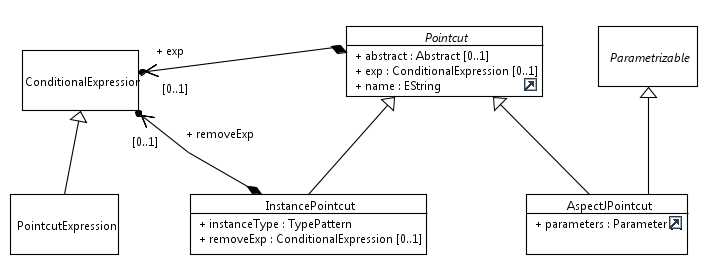
\includegraphics[width=\textwidth] {images/pc.png}
   \label{fig:shapes}
\label{fig:ip}
\caption{Instance pointcut static structure}
\end{figure}

Instance pointcuts can be compiled to various AO-languages, for our prototype we chose AspectJ as the target language. A pseudo-code of the generator template for instance pointcuts is shown in Listing \ref{lst:ip2aj}. 

\begin{lstlisting}[float=H, caption={Code generation templates for instance pointcut to AspectJ generation }, label={lst:ip2aj}]
Enumeration ExpressionType {SELECT, REMOVE}
generate(InstancePointut pc){
	if(pc.isAbstact){
		'abstract pointcut' pc.name'('pc.instanceType 'instance)'
		'Set<'pc.instanceType'>' pc.name'_set'
	}
	else{
		'Set<'pc.instanceType'>' pc.name'_set = new TreeSet<'pc.instanceType'>();'
		generateAspectJCode(pc, SELECT);
		if(pc.removeExpression != null)
			generateAspectJCode(pc, REMOVE);
  }
}	
generateAspectJCode(InstancePointcut pc, ExpressionType eType){
	String pcname, setOperation, setName = pc.name + '_set';
	PointcutExpression expTemp;
	switch(eType){
		case REMOVE:{
			pcname = pc.name + '_remove';
			setOperation = 'remove';
			expTemp = pc.removeExp;
		}
		case SELECT:{
			pcname = pc.name;
			setOperation = 'add';
			expTemp = pc.exp;
		}
	}	
	if(exp.contains(ReturningStatement))	{
		 PointcutExpression newExp = expTemp.remove(ReturningStatement);	
		'pointcut' pcname'():' print(newExp) ';'
		'after() returning(' instanceType 'instance):' pcname'(){'		
	}
	else{
		'pointcut' pcname'('pc.instanceType 'instance):' print(expTemp) ';'
		'after(' pc.instanceType 'instance):' pcname'(instance){'	
	}
	'boolean flag ='setName.setOperation '(instance);
	 if(flag)
		print(instance  +' setOperation ');
	}'
}
\end{lstlisting}

\section{Application on Online Shop}
\todo[inline]{this section will include sequence diagrams and advanced instance pointcuts for showing their benefits....}

\section{Compilation of Instance Pointcuts}
\todo[inline]{AspectJ code generation}
\todo[inline]{Generation of instance pointcut related hooks in the form of aspectj pointcuts, such as add/remove operations to the instance pointcut set}
\missingfigure{compilation algorithm?}

\section{Related Work}
\section{Discussion}
\section{Conclusion and Future Work}
\todo[inline]{keep it short}

%\section{The Binding Language}
%
%Instance pointcuts and adapter declarations are language concepts and ideally every aspect-oriented language can be extended to host them. We have implemented a prototype in AspectJ. While we have extended the syntax of AspectJ for instance pointcuts and adapter declarations, we have reused AspectJ's join-point model in instance pointcut expressions.  We will discuss possible extensions in other well known AO-languages at the end of this section. 
%
%\begin{figure}
%\centering
%\subfigure[Shapes Hierarchy]{
   %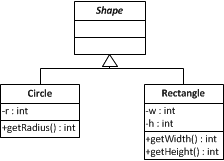
\includegraphics[width=0.4\textwidth] {images/shapes.png}
   %\label{fig:shapes}
 %}
%\qquad
 %\subfigure[ShapeInfo and used interfaces]{
   %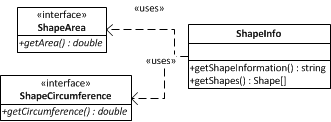
\includegraphics[width=0.4\textwidth] {images/shapeint.png}
   %\label{fig:shapesi}
 %}
%\label{fig:example1}
%\caption{Shapes Example}
%\end{figure}

%\subsection{Basic Language Features}
%We will explain the basics of the language with the help of a simple example. In Figure \ref{fig:shapes} a simple hierarchy of shapes is shown. The abstract class \texttt{Shape} has two subtypes called \texttt{Circle} and \texttt{Rectangle}. The interfaces provided by these classes can be seen in the figure. The \texttt{ShapeInfo} class shown in Figure \ref{fig:shapesi} collects the area and the circumference information of a given \texttt{Shape} using \texttt{ShapeArea} and \texttt{ShapeCircumference} interfaces, which are not implemented by any of the classes in the \texttt{Shape} hierarchy. 
%
%In Listing \ref{lst:circle} an simple instance pointcut that selects \texttt{Circle} instances and an adapter using that pointcut is defined. The name of the instance pointcut (line 2) is \textbf{\texttt{circles}} and the instance type is shown in Java generics syntax as \texttt{\textbf{<Circle>}}. The \texttt{call} primitive pointcut selects the join points where a new \texttt{Circle} object is created,then \texttt{\textbf{returning(instance)}} binds the returned \texttt{Circle} instance to the \emph{implicit variable} \texttt{\textbf{instance}}. The complete set of features of instance pointcuts will be discussed in Section \ref{sec:ip}. The adapter declaration (line 4), defines an adapter called \texttt{CircleAdapter} which implements \texttt{ShapeArea} and \texttt{ShapeCircumference} interfaces, indicated inside the curly braces. After the \texttt{\textbf{adapts}} keyword we declare which set of object we would like to adapt, in this case the set of objects selected by the \texttt{circles} pointcut. In the body of an adapter declaration, the implementation of the declared interfaces is given. Notice the \texttt{\textbf{adaptee}} keyword in the method bodies (lines 7, 12). The \texttt{adaptee} keyword refers to the object that's being adapted, in this case a \texttt{Circle} object, therefore can access its methods. 
%
%\begin{lstlisting}[float=tb, caption={An instance pointcut selecting Circle objects and an adapter declaration using this pointcut}, label={lst:circle}]
%aspect ShapeAdapterAspect{
	%instance pointcut circles<Circle> : call(* Circle.new(..)) && returning(instance);
%
	%declare adapter: CircleAdapter{ShapeArea, ShapeCircumference} adapts circles{
		%public double getArea()
		%{
			%return Math.PI*adaptee.getRadius()*adaptee.getRadius();
		%}
				%
		%public double getCircumference()
		%{
			%return 2*Math.PI*adaptee.getRadius();
		%}
	%}
%}
%\end{lstlisting}
%
%\subsection{Adapters}
%
%\subsection{Adapter Hierarchies}
%In this section we will add a new required interface to the example presented in Figure \ref{fig:example1}, called \texttt{ShapeColor}. This interface has a \texttt{getColor()} method, which returns \texttt{RED} if the area of the shape is smaller than \texttt{40} and \texttt{BLUE} for the rest. 
%
%\begin{lstlisting}[float=tb, caption={An Adapter Hierarchy}, label={lst:adaphier}]
%aspect ShapeAdapterAspect{
	%instance pointcut shapes<Shape> : call(* Shape+.new(..)) && returning(instance);
	%
	%declare adapter: abstract ShapeAdapter{ShapeArea, ShapeCircumference, ShapeArea} adapts shapes{
		%public String getColor(){
			%if(this.getArea() < 40)
				%return ``RED'';
			%else
				%return ``BLUE'';
		%}
	%}
%
	%declare adapter: CircleAdapter extends ShapeAdapter adapts shapes<Circle>{
		%//Implementation of ShapeArea and ShapeCircumference
	%}
	%declare adapter: RectangleAdapter extends ShapeAdapter adapts shapes<Rectangle>{
		%//Implementation of ShapeArea and ShapeCircumference
	%}
%}
%\end{lstlisting}
%
%In Listing \ref{lst:adaphier} an adapter hierarchy is shown. We have modified the instance pointcut to capture all \texttt{Shape} instances including instances of its subtypes using the ``+'' operator of AspectJ(line 2). The implementation of the \texttt{ShapeColor} interface does not depend on the instance type. We provide the implementation of this interface in an \textbf{abstract adapter} called \texttt{ShapeAdapter}(line 4) , which adapts all the \texttt{Shape} objects that are created. An adapter is declared abstract by placing the \texttt{abstract} modifier before its name. \emph{An abstract adapter can have unimplemented methods, whereas a concrete adapter had to implement all the unimplemented interface methods it declares and inherits.} Since \texttt{ShapeAdapter} is abstract it does not have to implement \texttt{ShapeArea} and \texttt{ShapeCircumference}, however it can refer to these interfaces' methods, as seen in line 6.  Abstract adapters cannot be instantiated, therefore it is necessary to have sub-adapters that are concrete.
%
%The concrete adapters extending \texttt{ShapeAdapter} are \texttt{CircleAdapter} (line 13) and \texttt{RectangleAdapter} (line 16). There are two things to notice in these sub-adapter declarations. First is that they do not declare any interfaces, that information is inherited from \texttt{ShapeAdapter} declaration. The second is the way instance pointcut \texttt{shapes} is refined. \emph{Instance pointcuts store the dynamic types of instances.} The statement \texttt{\textbf{shapes<Circle>}} selects a subset of \texttt{Shape} objects which have the dynamic type \texttt{Circle}. This refinement mechanism lets us create a \texttt{CircleAdapter} without writing a new pointcut which explicitly selects \texttt{Circle} instances, also by refining the same pointcut used in the super-adapter we ensure the set of \texttt{Circle} objects are a subset of \texttt{Shape} objects selected by \texttt{shapes} instance pointcut.
%
%\textbf{\textcolor[rgb]{1,0,0}{I think we should discuss whether we allow using a different pointcut in the sub-adapters.}}
%
%\subsection{Adapter Instantiation and Retrieval}
%While adapters are widely used to resolve incompatible interface problem, they introduce a cross-cutting concern to the which we identify as \emph{adapter instantiation concern}. In an OO-approach  the \texttt{ShapeInfo}(Figure \ref{fig:shapesi}) class has to create or reuse a \texttt{CircleAdapter} whenever it wants to get the area of a \texttt{Circle} object. In such a small example this does not cause a hindrance. However if we increase the size of this problem into a thousand \texttt{Shape} instances and increase the number of interfaces ShapeInfo has to deal with to 20, then instantiation of the right adapters for the right shapes and managing these adapters is not so trivial anymore. 
%
%Instance pointcuts and adapters declarations provide a declarative way for matching instances with the appropriate adapters. When an instance pointcut matches an instance and there's a concrete adapter declaration for that instance pointcut, the adapter instance containing the matching instance is automatically created. The automatic creation of adapters is an implicit behavior and it modularizes the adapter instantiation concern. 
%

\end{document}


%Software evolution requires integration of new components with the old ones. In an
%ideal component-based system, this integration should be seamless meaning 
 %the legacy components remain untouched and the interface of the new component is fully compatible with the existing interfaces. 
%Unfortunately such systems do not exist; as a result the integration is seldom
%seamless. Throughout the paper we will refer to the integration of two software components as a
%\emph{binding}. 
%
%We have defined three major challenges regarding binding. 
%\begin{enumerate}
  	%\item When components evolve, the links between them
	%must be re-established. 
 	 %\item When adding unforeseen functionality to a system, no explicit hooks
 	 %exist for attaching the new component. 
	%\item The interface of the components is not compatible and they should be adapted.
%\end{enumerate}
%
%Handling the first challenge requires a \emph{maintainable} way of expressing binding. It is possible to program binding according to some foreseeable evolution scenarios. However in today's component-based systems, third-party software is widely used. So when the interface offered by a third-party software changes, it is necessary to re-program the binding. \emph{Reusable binding structures} and expressing binding in a \emph{concise} manner is then valuable to reduce this programming effort.
%
%Handling the second challenge requires a means to expose certain information in an
%application's control flow and inject additional behavior to the control flow. Context exposure can be done via object-oriented programming(OOP), by providing classes which store and expose context information. Injecting additional behavior can be achieved via design patterns like dependency injection or decorator. However these methods are valid for planned extensions, and they will not be sufficient when a new component needs to access an unexposed context. Another issue is linked to the nature of binding two components. Since components need to be connected through possibly multiple points the \textbf{binding concern} becomes cross-cutting. It has been shown that OOP is not effective in modularizing such cross-cutting concerns.  
%
%Handling the third challenge requires a means to express the mapping between components. In this paper we present new language mechanisms to express such mappings and provide improvement on the solutions of the first two challenges. Our approach consists of two language concepts that work together; \emph{instance selectors} and \emph{adapter declarations}. 
%
%In the original GoF book, Adapter Pattern's purpose is defined as ``converting the interface of a class into another interface clients expect. Adapter lets classes work together that could not otherwise because of incompatible interfaces''. Adapters are an important part of a component-based system, since they are the building blocks of binding. 
%
%Our approach is designed as an addition to Aspect-Oriented Programming (AOP)\textbf{(?)}. AOP is used to modularize crosscutting
%concerns and with its 'weaving' mechanism, it is possible to change the behavior or the structure of an implementation without altering the
%implementation itself. These properties of AOP make it a desirable candidate for modularizing the binding concern.
%
%AOP is effective for achieving loose-coupling. It
%can capture information or inject behavior from a component without being
%acknowledged. AOP also facilitates the OO way of loose-coupling, which done via
%interfaces. It is possible to declare subtypes of an interface and provide the
%subsequent implementation in an aspect.  AOP is also efficient in localizing a concern. So when two components are bound using
%AOP, the binding implementation will be in one place. This is an important
%property for maintaining the modules providing loose-coupling. 
%
%\textcolor[rgb]{0.50,0.50,0.50}{A pointcut is a program construct that selects join points and expose context at
%those points \textbf{(AspectJ in Action book)}. Hence by using pointcuts we can
%define entry points to a system to inject new behavior. Of course this approach
%is limited with the expressiveness of the join-point model of the AO-language. }
%
%However implementation of adapters in current AOP approaches is type invasive. In AspectJ Adapter Pattern is implemented via inter-type declarations which alter the type system by making the adaptee implement a certain interface. This changes the type hierarchy of the adaptee. Also the Adapter Pattern disappears into the AspectJ syntax, which diminishes the visibility of the pattern. CaesarJ has an explicit syntax for defining adapters, which are referred to as wrappers in CaesarJ. However CeaserJ, although it gives great power over separation of concerns, tend to become too fragmented, hurting maintainability. 


%\begin{algorithm}[H]
%\SetAlgoLined
%\SetKwInOut{Input}{input}\SetKwInOut{Output}{output}
%\SetKwData{pcname}{\textbf{pc.name}}
%\SetKwData{pc}{\textbf{pc}}
%\SetKwData{itype}{\textbf{pc.instanceType}}
%\SetKwData{pcset}{instanceSet}
%\SetKwData{pcexp}{\textbf{pc.selectExpression}}
%\SetKwData{pcrem}{\textbf{pc.removeExpression}}
%\SetKwData{ret}{\textbf{returning}}
%\SetKwFunction{set}{CreateSet}
%\SetKwFunction{add}{Add}
%
%\Input{Instance Pointcut \pc}
%\Output{AspectJ code}
%\BlankLine
%
%\eIf{\pc is abstract}
%{
	%abstract pointcut \pcname ( \itype instance )\;
%}
%{
	%\pcset$\leftarrow$\set{\pcname\_Set}\;%TreeSet \pcname\_Set  = TreeSet()\;
	%\eIf{\pcexp contains \ret}
	%{
		%pointcut \pcname{} : \pcexp without \ret declaration\;
		%after() returning(\itype instance): \pcname{} \\
			%\Indp{\pcset$.$\add{instance}}
	%}
	%{
		%pointcut \pcname{\itype instance} : \pcexp;
		%after(\itype instance): \pcname{instance} \\
			%\Indp{\pcset$.$\add{instance}}
	%}
%
%}
%
%
%\caption{Compilation of instance pointcuts to AspectJ code}
%\label{alg:ip}
%\end{algorithm}
